\section{Estimation} \label{chap:results}
% Matching procedure (test change)
Based on the treatment/control assignment described in Section \ref{chap:data}, we match treated to control firms based on their previous employment and credit rating patterns. The outcome of interest is the mean difference in log employment evolutions from 2014-2015 and 2014-2016 between the two groups (semi-elasticity of employment w.r.t. the minimum wage). We apply large-sample bias correction and use AI standard errors, which factor in matching uncertainty \citep{Abadie2003,Abadie2006}.

% Covariate imbalance
Table (?) shows why the matching procedure is required. In particular, the second to last column shows that there are substantial differences between the treated and control sectors in their employment patterns and credit ratings. These differences are not constant over time, indicating that analyses which do not take this into account risk picking up this trend rather than a causal effect of the minimum wage introduction, particularly given that we expect the minimum wage effect to be small in size. The final column shows that our matching procedure deals with this issue quite effectively, ensuring that we are comparing firms that are on a similar growth trajectory (past employment) and are assumed to have similar prospects (credit ratings). Similarities in the mean might still mask differences along the rest of the distribution. In Figure \ref{fig:sumStats}, we show that the distribution of the six matching variables is very similar for the treated (solid line) and matched (dotted) observations. The same cannot be said for the raw controls (dashed), where especially for employment we observe considerable differences in densities.

\begin{figure}[htbp]
    \centering
    \caption{Distribution of the matching variables}
    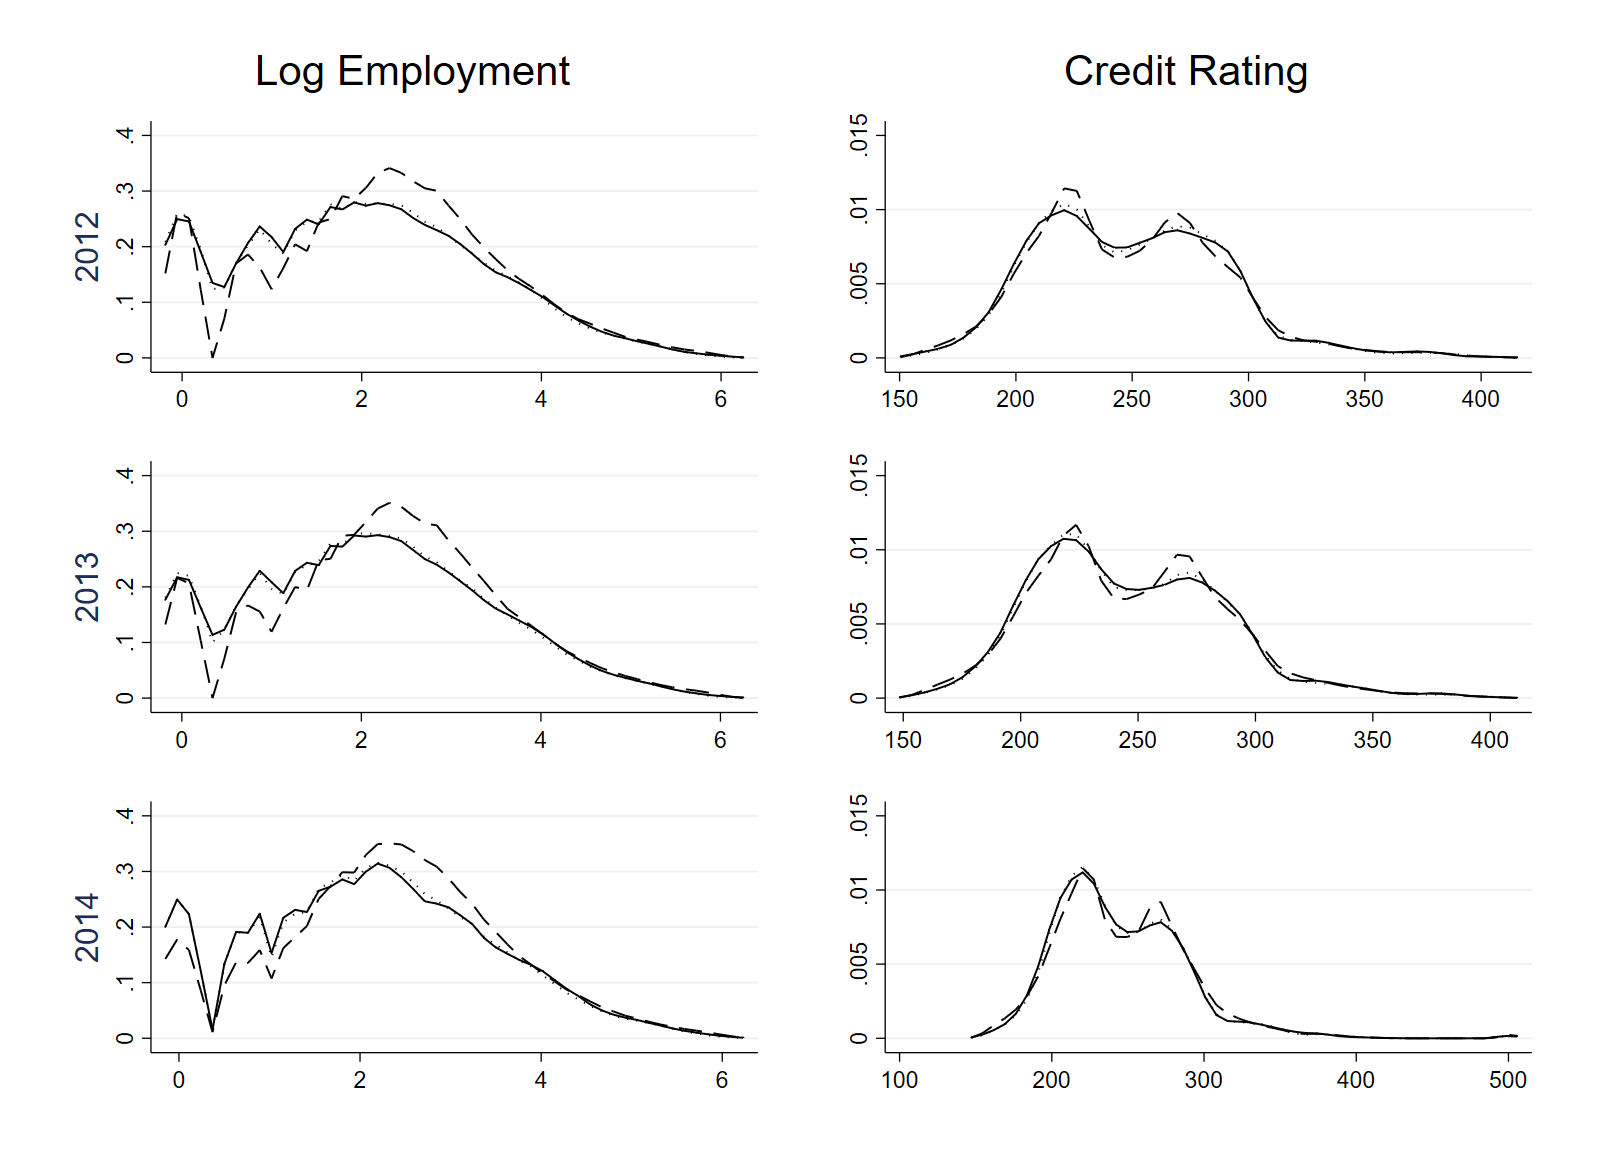
\includegraphics[width=0.70\paperwidth]{Images/summaryStats_graphs.png}
    \label{fig:sumStats}
    \caption*{Solid line: density of the treated observations. Dashed line: density of the full set of control observations. Dotted line: density of the matched set of control observations.}
\end{figure}
% Reference year/OLS
Table \ref{table:mainResults} shows the main results under different scenario's. Columns (1) and (2) provide estimates from a simple OLS regression where we include the matching variables as predictor. We have two years of post-intervention data and have chosen to use 2014 as reference point for both. That is, instead of comparing 14-15 and then 15-16, both are expressed relative to 2014. In the end, we are interested in the effect of the treatment, not necessarily whether there is a significant difference between 15 and 16.\footnote{The sample is restricted to be identical in both years.} As a result, the estimates represent the full effect up to that year and should not be added together.

% Main Results
% Replication: ctrl+F #mainResultsTable
\begin{table}[htbp]\centering
\caption{Employment and Turnover Effects}\label{table:mainResults}
\begin{threeparttable}
\begin{tabular}{l|cc|cc}
\toprule
&\multicolumn{2}{c|}{East}&\multicolumn{2}{c}{West}\\
&Emp&Turn & Emp&Turn\\
&(1)&(2)&(3)&(4)\\
\midrule
$\Delta$ Growth 14-15 &-.005& -.001& .002 & .011\\
&(.002)\sym{**}& (.004)& (.004) & (.006)\sym{**} \\
$\Delta$ Growth 14-16 &-.008& -.003& .001 & .033\\
&(.003)\sym{**}& (.006)& (.006) & (.009)\sym{***} \\
\midrule
\# of treated &5654& 3981& 1562 & 1115\\
\# of controls &39012& 27787& 39012 & 27788\\
\# of controls used &8008& 2876& 2699 & 1090\\
\midrule
SDM 13-14 &.02& -.01& .02& .02\\
Level Diff 2013&0& -.01& .01& 0\\
Trend 2011-2014&\checkmark&\checkmark&\checkmark&\checkmark \\
Specification & Base & U & Base & Prod $+$ U\\
\bottomrule
\end{tabular}
\begin{tablenotes}
\item $\Delta$ Growth is the difference in growth between the treated and control. SDM refers to the standardised difference in means. 
Level Diff 2013 indicates the difference in log levels between treated and control in 2013. 
Trend indicates how this level difference evolved between 2011 and 2014.
Specification shows which matching specification scored best at the evaluation criteria. Prod: match also on 2014 labour productivity of firm (emp/turn),
U: ... on the unemployment rate within state.
\item Matching uncertainty robust AI standard errors in parentheses \citep{Abadie2006}.
\item \emph{Stars}: \sym{*} \(p<0.1\), \sym{**} \(p<0.05\), \sym{***} \(p<0.01\)
\end{tablenotes}
\end{threeparttable}
\end{table}

% Size Results
% Replication: ctrl+F #sizeResultsTable
\begin{table}[htbp]\centering
\caption{Employment and Turnover Effects - Micro and Small Enterprises}\label{table:sizeResults}
\begin{threeparttable}
\begin{tabular}{l|cccc|cccc}
\toprule
&\multicolumn{4}{c|}{East}&\multicolumn{4}{c}{West}\\
&\multicolumn{2}{c}{Micro}&\multicolumn{2}{c|}{Small}&\multicolumn{2}{c}{Micro}&\multicolumn{2}{c}{Small}\\
&Emp&Turn & Emp&Turn&Emp&Turn & Emp&Turn\\
&(1)&(2)&(3)&(4)&(5)&(6)&(7)&(8)\\
\midrule
$\Delta$ Growth 14-15 &-.009& -.006&.002& -.005& -.002 & .026& .019 & .016\\
&(.004)\sym{**}& (.005)&(.003)& (.005)& (.008) & (.01)\sym{***}& (.006)\sym{***} & (.009)\sym{*} \\
$\Delta$ Growth 14-16 &-.018& .003&-.001& -.008& -.007 & .046& .034 & .043\\
&(.006)\sym{***}& (.008)&(.005)& (.008)& (.011) & (.018)\sym{**}& (.009)\sym{***} & (.013)\sym{***} \\
\midrule
\# of treated &2875& 1821&2091& 1401& 552 & 342& 665 & 457\\
\# of controls &39009& 27785&39012& 27787& 39009 & 27787& 38908 & 27788\\
\# of controls used &3001& 1579&2534& 1283& 512 & 328& 610 & 471\\
\midrule
SDM 13-14 &-.02& -.01&.09& -.01& -.01& -.01& .02& .03\\
Level Diff 2013&-.27& -.27&.01& .02& -2.4& -.08& .16& .02\\
Trend 2011-2014&\checkmark&\checkmark& $\times$&\checkmark&?&$\times$&\checkmark&? \\
Specification & MJ & MJ & Base & Base & MJ & Prod $+$ U&Prod $+$ U&Base\\
\bottomrule
\end{tabular}
\begin{tablenotes}
\item $\Delta$ Growth is the difference in growth between the treated and control. SDM refers to the standardised difference in means. 
Level Diff 2013 indicates the difference in log levels between treated and control in 2013. 
Trend indicates how this level difference evolved between 2011 and 2014.
Specification shows which matching specification scored best at the evaluation criteria. Prod: match also on 2014 labour productivity of firm (emp/turn),
U: ... on the unemployment rate within state.
MJ: ... on the share of mini-jobbers within state.
\item Matching uncertainty robust AI standard errors in parentheses \citep{Abadie2006}.
\item \emph{Stars}: \sym{*} \(p<0.1\), \sym{**} \(p<0.05\), \sym{***} \(p<0.01\)
\end{tablenotes}
\end{threeparttable}
\end{table}



% Main Results/OLS
What we find is that there is a statistically significant negative impact overall, but it is relatively small. That is, the introduction of the national minimum wage reduced employment rates in the highly affected sectors by just 1 percent, much less than predicted ex ante (see Section \ref{chap:discussion}). Moreover, this result is not homogeneous across sectors. For example, the OLS results in column (2) suggest that the restaurant and fastfood sector benefited from the new minimum wage, with employment increases of 4\% in 2015, rising to 6\% in 2016.

% Main Results/Why we match (repeat)
However, these results may be driven by pre-existing trends, as well as observable and unobservable differences between firms in the treated and untreated industries. In this non-randomized experiment, there is very little we can do against the latter, but our matching procedure should at least ensure that we are comparing firms with a similar past and in a similar financial situation. 

% Main Results/Matching outcomes
Results are presented in columns (3) and (4). Qualitatively, the results remain the same. I.e. we still estimate a small negative impact overall (-1.1\% in 2016) and a positive one in the restaurant sector. The latter does become about 20\% smaller, suggesting employment in the restaurant sector increased by 3\% in 2015, up to 5\% in 2016. In an alternative specification, we omit the credit ratings and focus on matching pretreatment employment evolutions. The impact on the restaurant sector remains essentially unchanged, with respectively a three and a five percent increase (column 6). The estimated impact across all affected sectors becomes markedly larger, rising to a 1.5\% employment loss by 2016 (column 5).


% Results by firm size (overall)
Table (??) shows results per firm size. Starting with the results across all sectors in columns (1)-(3), we see that the only significant effect is found among the smaller firms (10-49 employees), where we see a drop of 1.6\%.\footnote{The effects are identical for micro firms of less than ten employees.} The effect on medium sized firms (50-249) is smaller (-0.9\%) and only significant at 10\%. Large firms (250+) even appear to have benefited from the minimum wage introduction. However, the estimate is based on just 57 treated and 48 control firms and only significant at 10\%.

In the restaurant sector, a similar pattern can be observed. The only significant effect is found in the micro firms (1-10 employees), where we see an increase of 7.5\% by 2016. The effect remains positive for small firms (1.5\%), but loses significance. Medium sized firms appear unaffected, with very imprecise estimates centered around -1\%. There are insufficient large firms to perform a matching exercise there.
